\documentclass[a4paper,12pt]{report}

\usepackage{alltt, fancyvrb, url}
\usepackage{graphicx}
\usepackage[utf8]{inputenc}
\usepackage{float}
\usepackage{hyperref}

% Questo commentalo se vuoi scrivere in inglese.
\usepackage[italian]{babel}

\usepackage[italian]{cleveref}

\title{Report progetto\\``Puzzle Bobble''}

\author{Riccardo Pepe\\
		Beatrice Barba}
\date{\today}


\begin{document}

\maketitle

\tableofcontents

\chapter{Analisi}

\section{Requisiti}

Il software che si vuole realizzare mira alla costruzione di un gioco rompicapo su livelli ispirato al famoso ``Puzzle Bubble''. 
Il gioco consiste nel liberare, tramite un cannone al cui interno è posizionata una pallina dal colore casuale, un tabellone che presenta un pattern delle suddette sfere.  Per superare il livello bisognerà liberare quest'ultimo dalle palline colorate prima che le sfere superino un punto limite e quindi venga dichiarato il game over.


\subsubsection{Requisiti funzionali}
\begin{itemize}
	\item Quando si formano degli agglomerati di minimo 3 sfere dello stesso colore, queste esploderanno incrementando il punteggio, facendo cadere anche le altre sottostanti che si ancoravano ad esso.
	\item Per liberare il tabellone è necessario far esplodere tutte le palline presenti.
	\item Dopo un determinato numero di colpi la difficoltà del giocatore nel liberare l'intero tabellone verrà incrementata gradualmente.
	\item Al completamento di ogni livello il gioco si occuperà di salvare automaticamente lo stato del gioco
\end{itemize}

\subsubsection{Requisiti non funzionali}
\begin{itemize}
	\item Il gioco deve rimanere fluido in tutte le sue fasi
\end{itemize}

\section{Analisi e modello del dominio}

Il gioco si compone di un tabellone rettangolare dove, nella parte alta, vengono posizionate delle palline in base ad uno schema; queste, in base al loro colore, possiedono punteggi differenti che, una volta esplose, incrementeranno il punteggio del giocatore. Nella parte inferiore dell'area di gioco è situato al centro un cannone al cui interno è presente una sfera dal colore casuale. L'utente può modificare la direzione del cannone e decidere dove sparare la pallina, tenendo conto che essa può rimbalzare sulle pareti laterali del rettangolo. Durante la partita, dopo un determinato numero di colpi effettuati, dalla parte superiore del tabellone inizierà a scendere un muro che avvicinerà le palline al cannone, aumentando così la difficoltà del livello. Il game over avviene quando le sfere inesplose superano una determinata linea di demarcazione. 

\begin{figure}[H]
\centering{}
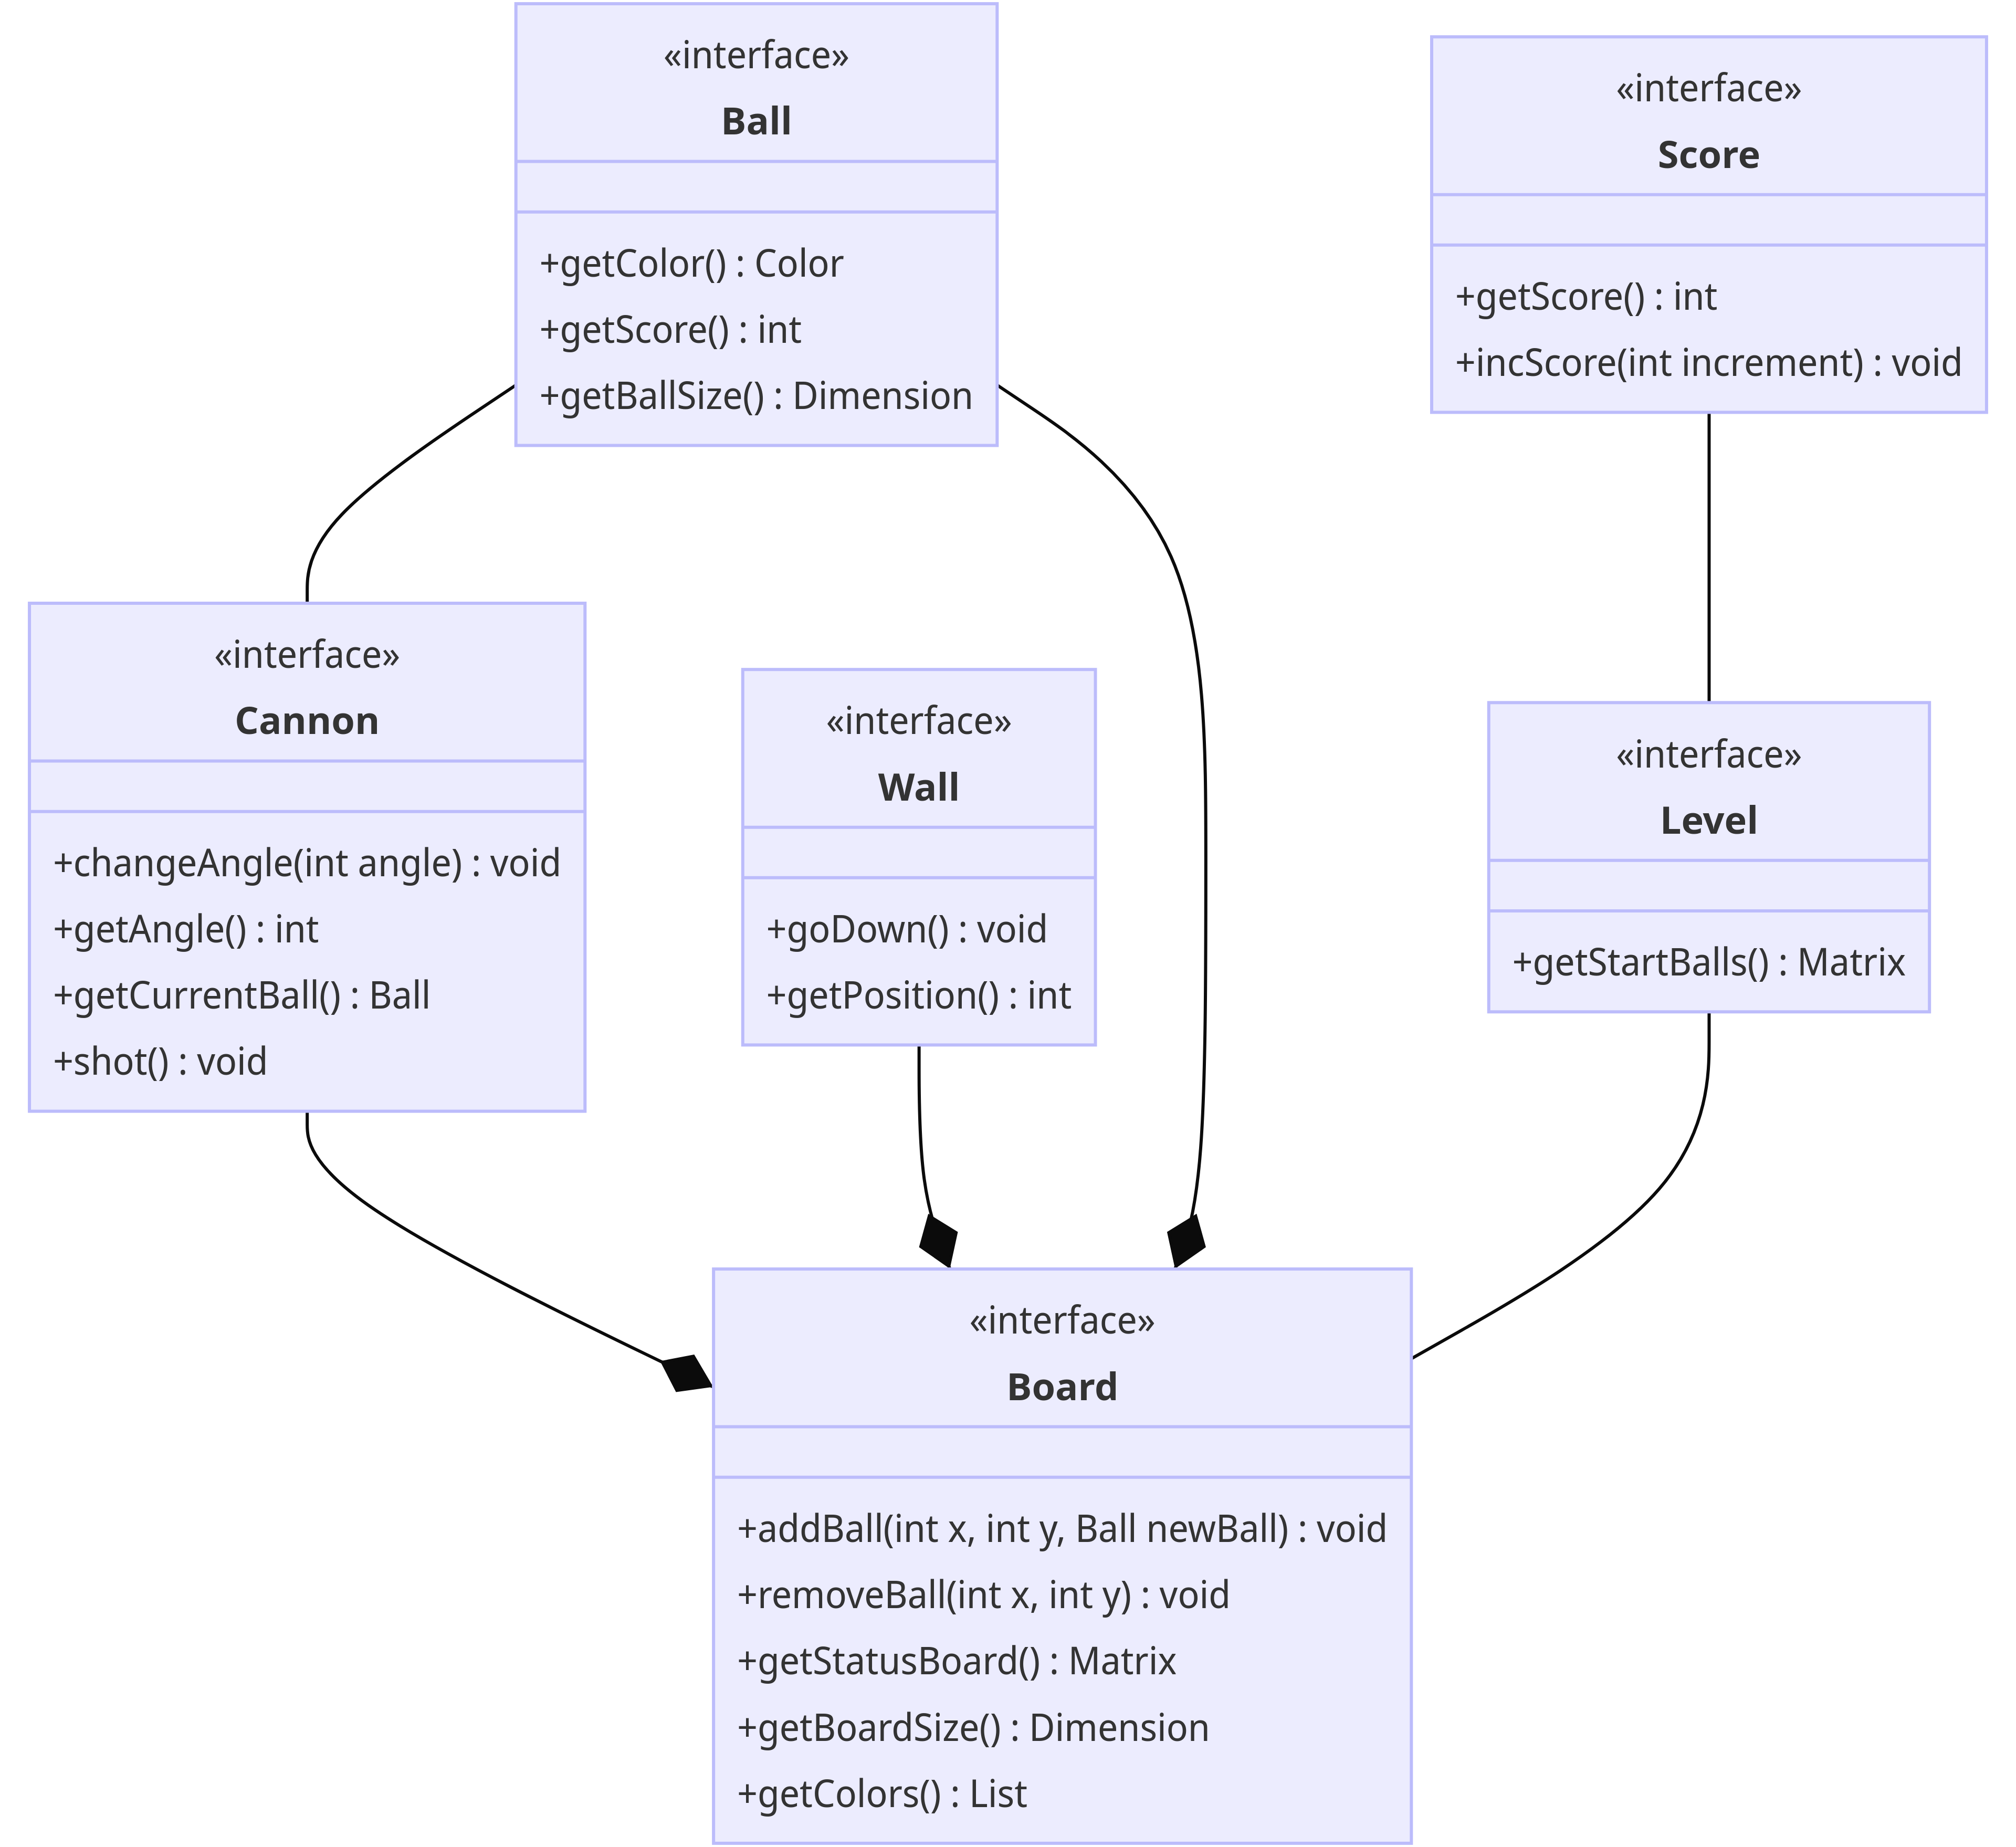
\includegraphics[width=0.95\textwidth]{img/Diagramma_UML_Analisi_Dominio}
\caption{Schema UML dell'analisi del problema, con rappresentate le entità principali ed i rapporti fra loro}
\label{img:analysis}
\end{figure}

\chapter{Design}

\section{Architettura}

Si è scelto per questo progetto di utilizzare il pattern \textbf{MVC} dividendo in 3 macro  categorie le classi architetturali: 
l'interfaccia \textbf{Model} racchiuderà tutta la logica del gioco analizzata nella fase di analisi del dominio; la  macro sezione Control sarà composta da due interfacce una sarà \textbf{Gameloop} dove verrà gestito il vero e proprio game, mentre una seconda a cui verrà affidato il compito di gestire la creazione dei livelli e di istanziare il Gameloop, detta \textbf{GameState}. Infine per la terza macro categoria, la View, ci saranno due interfacce una per catturare gli input, che si chiamerà \textbf{Input}, e la seconda per visualizzare sullo schermo lo stato del gioco, detta \textbf{Output}.


Il Model interagirà solo con il Gameloop in modo da incapsulare la logica del gioco e dei suoi componenti  in un unica interfaccia; il Gameloop e il GameState saranno collegati all'Input e all'Output in modo da tenere separate la View e il Model in modo che in caso di necessità di cambiare a libreria della grafica on si debba modificare  a cascata l'intera architettura. 

\begin{figure}[H]
\centering{}
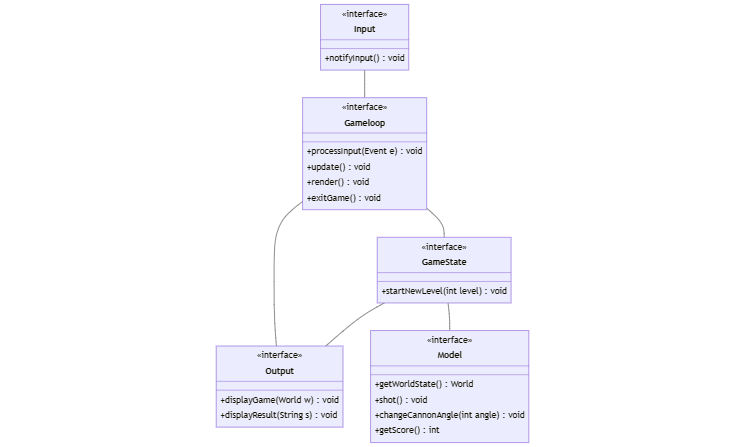
\includegraphics[width=\textwidth]{img/Diagramma_UML_Architettura}
\caption{Schema UML architetturale di Puzzle Bobble. Le interfacce \texttt{Gameloop e GameState} sono il controller del sistema, mentre \texttt{Input} ed \texttt{Output} sono le interfacce che mappano la view. \texttt{Model} è autoesplicativa.}
\label{img:Diagramma_UML_Architettura}
\end{figure}

In \Cref{img:Diagramma_UML_Architettura} è esemplificato il diagramma UML architetturale.

\newpage
\section{Design dettagliato}

\subsection{Pepe Riccardo}

\subsubsection{Creazione delle palline}

\paragraph{Problema} In fase di sviluppo sono state individuate due tipologie di palline, una statica (posizionata sul muro superiore del tabellone) ed una dinamica (appena sparata). La pallina dinamica possiede le stesse proprietà e metodi di quella statica, con in aggiunta la gestione di un campo posizione. Inoltre ogni pallina possiede un colore, e da questo colore deriva l'attributo score, ovvero quanti punti vale quella pallina con quello specifico colore. A questo punto è necessario valutare una soluzione per evitare duplicazioni e ridondanze nel codice.


\paragraph{Soluzione} Appare chiaro che la pallina dinamica sia una specializzazione della pallina statica. Inoltre, dato che il numero di colori è molto inferiore rispetto alle ball che verranno effettivamente utilizzate, si è deciso di incapsulare la logica della creazione delle palline e quindi delle proprietà derivate dal colore in una factory, secondo il \textit{pattern factory method}.

\begin{figure}[H]
\centering{}
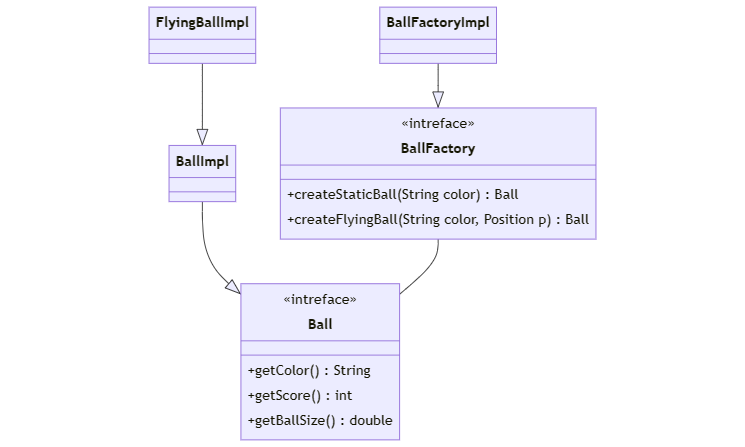
\includegraphics[width=\textwidth]{img/Diagramma_UML_Ball}
\caption{Rappresentazione UML del pattern Factory}
\label{img:Diagramma_UML_Ball}
\end{figure}

\subsubsection{Creazione del GameLoop}

\paragraph{Problema} Un videogioco richiede una gestione del flusso di gioco il più possibile fluida e costante. Quindi si rende necessario uno strumento che controlli il flusso e quindi gestisca le vari componenti dell'architettura in modo coordinato, senza esagerare nella richiesta di risorse alla macchina.

\paragraph{Soluzione} Il pattern gameloop è la soluzione che meglio si adatta a questa necessità. Inoltre permette di avere una frequenza di aggiornamento costante ed una gestione degli input efficiente.

\begin{figure}[H]
\centering{}
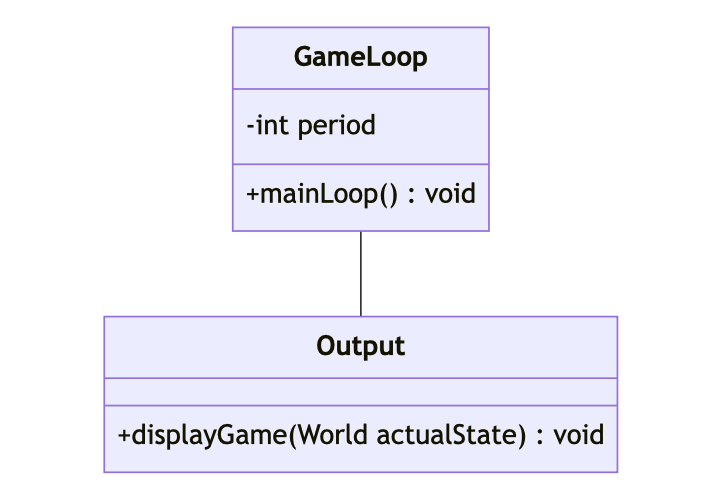
\includegraphics[width=\textwidth]{img/Diagramma_UML_GameLoop}
\caption{Rappresentazione UML del pattern GameLoop}
\label{img:Diagramma_UML_GameLoop}
\end{figure}

\subsubsection{Gestione degli input}

\paragraph{Problema} La gestione degli input deve essere il più possibile modulare e incapsulare al loro interno la logica dietro ogni singolo comando.

\paragraph{Soluzione} Il pattern Command si rivela adatto a questa situazione. Infatti incapsulando dentro una interfaccia Command la logica dietro un input permette di avere una maggiore manutenibilità e facilità di implementazione del codice. L'interfaccia Controller si occuperà di mettere in lista il comando e richiederne l'esecuzione. Questa soluzione si adatta particolarmente bene con il pattern GameLoop.

\begin{figure}[H]
\centering{}
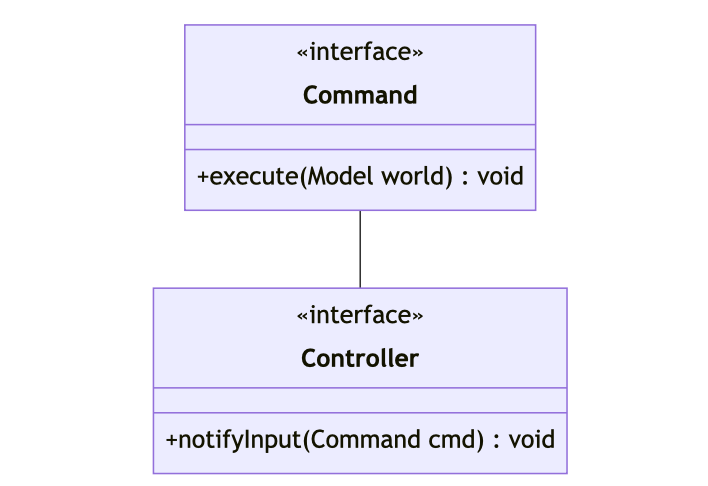
\includegraphics[width=\textwidth]{img/Diagramma_UML_Command}
\caption{Rappresentazione UML del pattern Command}
\label{img:Diagramma_UML_Command}
\end{figure}

\subsection{Barba Beatrice}

\subsubsection{Creazione del Model}

\paragraph{Problema} Durante la fase di sviluppo del dominio di gioco si è notato come esso fosse di elevata complessità, ma che solo poche funzionalità fossero necessarie per l'interazione tra tutta la logica del gioco e l'utente. È sorta la necessità di trovare un modo per separare la complessità del dominio dalle poche funzionalità strettamente necessarie per controllare l'avanzamento del gioco. 

\paragraph{Soluzione} Questo problema è risolvibile tramite il pattern Facade che si occupa proprio di creare una classe  intermedia in cui vengono racchiusi solo i metodi necessari e più semplici, racchiudendo la complessità e la logica nelle classi che istanzia. In questo caso la classe Model racchiude tutti gli oggetti degli elementi del gioco e richiama solo i metodi necessari all'utente lasciando tutta la complessità implementativa alle classi specifiche che implementano gli elementi.
\begin{figure}[H]
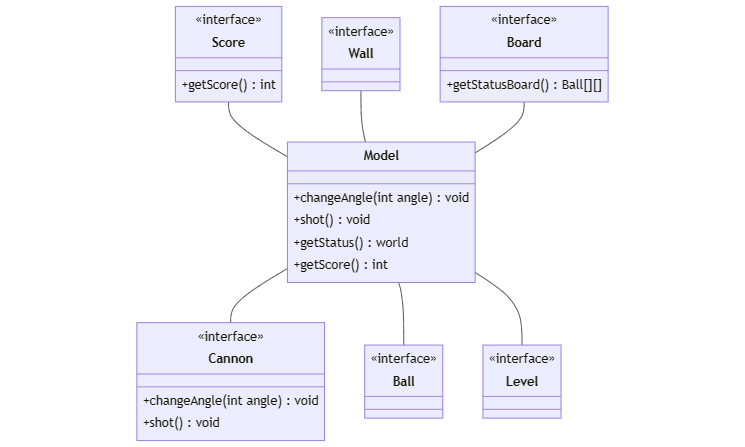
\includegraphics[width=\textwidth]{img/Diagramma_UML_Architettura_Model}
\caption{Rappresentazione UML del pattern Facade usato per il Model}
\label{img:Diagramma_UML_Architettura_Model}
\end{figure}

\subsubsection{Gestione Input/Output}

\paragraph{Problema} Per la gestione del gioco è necessario leggere e scrivere dal file system. Dato che svariati elementi dell'architettura utilizzeranno questa funzionalità sarà necessario passare a tutti il riferimento di esso. 

\paragraph{Soluzione} Questo problema è risolvibile tramite il pattern Singleton che si occupa di rendere una classe globale in modo da essere raggiungibile da tutte le classi che avranno bisogno di accedere al file senza dover creare tante istanze per lo stesso oggetto. 

\begin{figure}[H]
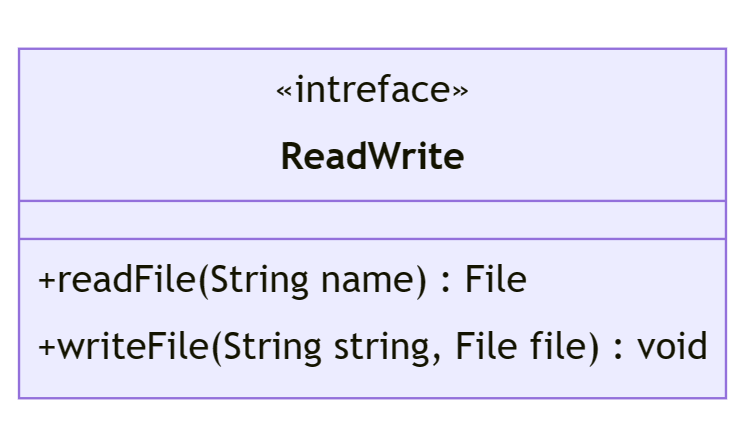
\includegraphics[width=\textwidth]{img/Diagramma_UML_Architettura_Singleton}
\caption{Rappresentazione UML del pattern Singleton usato per leggere e scrivere su file system}
\label{img:Diagramma_UML_Architettura_Singleton}
\end{figure}


\chapter{Sviluppo}
\section{Testing automatizzato}

Per effettuare i test automatizzati si è scelto di utilizzare JUnit e di testare solo le classi del Model.
Si è testata l'interfaccia Ball in base alla creazione delle palline diverse,FlyingBall e StaticBall, e nei getter che possiede; la classe Wall, Cannon e Score in base ai metodi delle loro interfacce, la classe Physics per verificare il funzionamento dei metodi per calcolare la traiettoria della pallina e dove dovesse essere posizionata nella Board; la classe Board per verificare il funzionamento dei metodi di aggiunta e rimozione delle palline dal tabellone, con molteplici test sulle varie dinamiche per la rimozione, le classi di scrittura e lettura dei file JSON, JSONParser e JSONReader e infine la classe Level in modo da verificare il corretto caricamento e la corretta trasformazione dei file JSON in matrici di palline.

\section{Metodologia di lavoro}

La fase di analisi e design dell'architettura è stata svolta insieme decidendo poi quali parti di ogni componente dell'arcchitettura dovesse fare ogni componente del gruppo in modo da fare entrambi una parte di View, una di Coontroller e una di Model. Dopo di che ognuno  ha operato per conto proprio, rimanendo comunque costantemente in contatto in modo da procedere in modo progressivo, spirale, nello sviluppo del gioco. 

Di comune accordo si è deciso di creare per ogni elemento del dominio un branch a parte, in modo da rilasciare una versione di essi nel main solo quando fosse stata completa e funzionante. 
Una volta sviluppate tutte le classi in singolo ci siamo incontrati  per poter controllare che le parti che devono comunicare fossero  ben amalgamente. 

\subsection{Pepe Riccardo}
Mi sono occupato delle classi: 
\paragraph{Model}
\begin{itemize}
\item {Ball,}
\item {BallFactory,}
\item {GameStatus,}
\item {Level,}
\item {Score,}
\item {Physics; }
\end{itemize}    
\paragraph{Controller} 
\begin{itemize}
\item {GameLoop,}
\item {Savestate,}
\item {WorldFormatter}
\end{itemize}  
  
\subsection{Barba Beatrice}
Mi sono occupata delle classi:
\paragraph{Model:} 
\begin{itemize}
\item {Board,}
\item {Wall,}
\item {Cannon,}
\item {Model; }
\end{itemize}
\paragraph{Controller}
\begin{itemize}
\item {GameState}
\end{itemize}  

\subsection{Entrambi}
Ci siamo occupati delle classi: JSONParser, JSONReader, FXMLController, Output, ViewController, View, App;

\section{Note di sviluppo}

\subsection{Pepe Riccardo}
\subsubsection{Uso  di lambda expression}
\centering
\url{https://github.com/rickpepp/OOP22-puzbob/blob/c78d6b0cd3700a3df4e830c6d105e520ab5d59e1/src/main/java/it/unibo/puzbob/controller/GameLoop.java#L79}

\subsubsection{Uso di JavaFX}
\centering
\url{https://github.com/rickpepp/OOP22-puzbob/blob/c78d6b0cd3700a3df4e830c6d105e520ab5d59e1/src/main/java/it/unibo/puzbob/view/FXMLController.java#L70}

\subsubsection{Uso della libreria org.json}
\centering
\url{https://github.com/rickpepp/OOP22-puzbob/blob/c78d6b0cd3700a3df4e830c6d105e520ab5d59e1/src/main/java/it/unibo/puzbob/model/JSONParser.java#L6}

\subsubsection{Uso dei Thread}
\centering
\url{https://github.com/rickpepp/OOP22-puzbob/blob/c78d6b0cd3700a3df4e830c6d105e520ab5d59e1/src/main/java/it/unibo/puzbob/view/ViewController.java#L5}

\subsection{Barba Beatrice}
\subsubsection{Uso di lambda expression}
\centering
\url{https://github.com/rickpepp/OOP22-puzbob/blob/c78d6b0cd3700a3df4e830c6d105e520ab5d59e1/src/main/java/it/unibo/puzbob/view/View.java#L133C31-L133C36}

\subsubsection{Uso  di JavaFX}
\centering
\url{https://github.com/rickpepp/OOP22-puzbob/blob/c78d6b0cd3700a3df4e830c6d105e520ab5d59e1/src/main/java/it/unibo/puzbob/view/FXMLController.java#L182}

\subsubsection{Uso di libreria org.json}
\centering
\url{https://github.com/rickpepp/OOP22-puzbob/blob/c78d6b0cd3700a3df4e830c6d105e520ab5d59e1/src/main/java/it/unibo/puzbob/model/JSONParserImpl.java#L27}

\subsubsection{Uso di Thread}
\centering
\url{https://github.com/rickpepp/OOP22-puzbob/blob/c78d6b0cd3700a3df4e830c6d105e520ab5d59e1/src/main/java/it/unibo/puzbob/model/ModelImpl.java#L76}

\begin{flushleft}
\chapter{Commenti finali}

\section{Autovalutazione}

\subsection{Pepe Riccardo}

Questo progetto ha richiesto una quantità di lavoro importante per il suo completamento. Sicuramente la qualità del tempo utilizzato nella realizzazione di questo lavoro non è sempre stata ottimale, l'utilizzo di qualche funzionalità avanzata di Java avrebbe sicuramente ridotto le quantità di ore di lavoro impiegate a favore di una maggiore qualità del prodotto finale. Questo progetto porta con se molti insegnamenti ed esperienza, in quanto le difficoltà apparse lungo il percorso non sono mancate. Tuttavia ritengo soddisfacente il risultato finale guardando il percorso effettuato.

\subsection{Barba Beatrice}
Nel complesso sono soddisfatta del lavoro svolto. Non sentendomi sicura delle mie conoscenze di Java all'inizio del progetto ho chiesto al mio compagno di poter avere le classi che, all'apparenza, mi sembravano meno complesse. Non sono ancora convinta che il carico di lavoro sia stato equo, ma durante lo sviluppo in solitaria mi sono accorta di come avevo sottovalutato alcuni metodi di alcune classi che ho avuto la possibilità di scegliere. Sono contenta però di aver realizzato io la classe Model, in quanto, per quanto non sia la classe ideale intermedia, ho voluto utilizzare le classi implementate dal mio compagno  leggendomele e non chiedendo direttamente a lui come utilizzarle. Avrei potuto fare sicuramente meglio, ma questo progetto mi è stato utile a capire concretamente cosa vuol dire creare un'applicazione dall'inizio alla fine in tutte le sue sfacettature oltre ad aver acquisito maggiori competenze con Java.

\section{Difficoltà incontrate e commenti per i docenti}
La difficoltà maggiore riscontrata è stata creare un intero progetto in due e non in quattro, poichè il carico di lavoro era stato pensato per essere svolto in gruppo e non in coppia.

\bibliographystyle{alpha}
\bibliography{report-PuzBob}
\end{flushleft}
\end{document}
